\documentclass[../main.tex]{subfiles}

\usepackage{nopageno} %Seitenzahlen auf richtiger Seite 

\usepackage[left=2cm, right=2cm, top=2cm, includehead, includefoot, headheight=17pt]{geometry}

\usepackage[utf8x]{inputenc}
\usepackage[english]{babel}
\usepackage{amsmath,amssymb,amsthm}
\usepackage{framed}
\usepackage{wasysym}
\usepackage[T1]{fontenc} %Silbentrennung 
\usepackage{color} %Farbe
\usepackage{graphicx}
\usepackage{float}%Grafik am gleichen Ort plazieren
%pdf. png. einfach eingliedern
\usepackage{subfigure} %Grafiken nebeneinander
\usepackage{pdfpages}
\usepackage{ulem} 	%\uuline{urgent}    % doppelt unterstreichen
%\uwave{boat}      % unterschlängeln
%\sout{wrong}       % durchstreichen
%\xout{removed}     % ausstreichen mit //////.

\usepackage{tikz}
\usetikzlibrary{trees}
\usetikzlibrary{plotmarks}
\usetikzlibrary{angles,quotes,babel}
\usetikzlibrary{shadings}
\usetikzlibrary{patterns}
\usetikzlibrary{matrix}
\usetikzlibrary{arrows}
\usetikzlibrary{calc}

\usepackage{pgfplots}
\usepackage{pgf-pie}
\pgfplotsset{compat=1.10}
\usepgfplotslibrary{statistics}
\usepgfplotslibrary{fillbetween}

\usepackage{tkz-euclide}
\usepackage{enumerate}
\usepackage{stmaryrd}
\usepackage{tabularx}
\usepackage{wrapfig}
\usepackage{epsdice}
\usepackage{multirow}
\usepackage{rotating}
\usepackage{pdflscape}
\usepackage{fancyhdr}

\pagestyle{fancy} %eigener Seitenstil
\fancyhf{} %alle Kopf- und Fußzeilenfelder bereinigen
\fancyhead[L]{} %Kopfzeile links
\fancyhead[C]{} %zentrierte Kopfzeile
\fancyhead[R]{} %Kopfzeile rechts
\renewcommand{\headrulewidth}{0.4pt} %obere Trennlinie
\fancyfoot[C]{\thepage} %Seitennummer
\renewcommand{\footrulewidth}{0.4pt} %untere Trennlinie

% Number spaces 
\newcommand{\CC}{\ensuremath{\mathbb{C}}}
\newcommand{\RR}{\ensuremath{\mathbb{R}}}
\newcommand{\QQ}{\ensuremath{\mathbb{Q}}}
\newcommand{\ZZ}{\ensuremath{\mathbb{Z}}}
\newcommand{\NN}{\ensuremath{\mathbb{N}}}
\newcommand{\LL}{\ensuremath{\mathbb{L}}}
\newcommand{\DD}{\ensuremath{\mathbb{D}}}
\newcommand{\WW}{\ensuremath{\mathbb{W}}}

%draw chemestry molecules 
\usepackage{chemfig} % https://mirror.ox.ac.uk/sites/ctan.org/macros/generic/chemfig/

\newcommand\vv[1]{%
	\begin{tikzpicture}[baseline=(arg.base)]
		\node[inner xsep=0pt] (arg) {$#1$};
		\draw[line cap=round,line width=0.45,->,shorten >= 0.2pt, shorten <= 0.7pt] (arg.north west) -- (arg.north east);
	\end{tikzpicture}%
} %command will render \vv{x} with an arrow aboth 

\renewcommand{\labelenumi}{\roman{enumi})}

\DeclareMathOperator{\ggT}{ggT}
\DeclareMathOperator{\sign}{sign}

%sections
\theoremstyle{plain}
\newtheorem{Thm}{Theorem}[section]
\newtheorem{Def}[Thm]{Definition}
\newtheorem{Prop}[Thm]{Proposition}

\theoremstyle{definition}
\newtheorem{lemma}[Thm]{Lemma}
\newtheorem{corollary}[Thm]{Corollary}
\newtheorem{claim}[Thm]{Claim}
\newtheorem{Proof}[Thm]{Proof}
\newtheorem{Ex}[Thm]{Example}

\newtheorem{Exercise}{ex}[section] %follow proper enum
\newtheorem{ex}[Exercise]{Exercise}
\newtheorem{Solution}{sol}[section]
\newtheorem{sol}[Solution]{Solution}

\theoremstyle{remark}
\newtheorem{remark}[Thm]{Remark} % follows thm enum

\newtheorem{comment}{Comment}[section] %follow comment enum
\newtheorem{notation}[comment]{Notation}
\newtheorem{reasoning}[comment]{Reasoning}
\newtheorem{Intpr}[comment]{Interpretation}

%some premmade with title (uterwise use \textbf{Title} ...)
\newenvironment{ThmWithTitle}[1]{%
	\begin{Thm}[\textbf{#1}]}{\end{Thm}}
\newenvironment{PropWithTitle}[1]{%
	\begin{Prop}[\textbf{#1}]}{\end{Prop}}
\newenvironment{ExWithTitle}[1]{%
	\begin{Ex}[\textbf{#1}]}{\end{Ex}}
\newenvironment{DefWithTitle}[1]{%
	\begin{Def}[\textbf{#1}]}{\end{Def}}
\newenvironment{RemarkWithTitel}[1]{%
	\begin{remark}[\textbf{#1}]}{\end{remark}}

%format of paragraph 
\renewcommand\paragraph{\@startsection{paragraph}{4}{\z@}%
	{-2.5ex\@plus -1ex \@minus -.25ex}%
	{1.25ex \@plus .25ex}%
	{\normalfont\normalsize\bfseries}}
\makeatother
\setcounter{secnumdepth}{4} % how many sectioning levels to assign numbers to
\setcounter{tocdepth}{4}    % how many sectioning levels to show in ToC

\newcounter{row} 
\renewcommand\therow{\alph{row}} %hier a,b,c etc. def und mit therow abrufbar

\newenvironment{aufz}
{\setcounter{row}{0}%
	\par\noindent\tabularx{\linewidth}[t]
	{\cdot{20}{>{\stepcounter{row}\makebox[1.5em][l]{\therow)\hfill}}X}} %bis max 20 Elemente nebeinander
}
{\endtabularx}


%biblio
\usepackage[]{biblatex}
\addbibresource{referenzenma.bib} 

%glossary
\usepackage{glossaries}
\usepackage{import}


\usepackage{rotating} % Include this package in the preamble

\newglossaryentry{hexokinase}{
	name={Hexokinase},
	description={An enzyme that catalyzes the phosphorylation of glucose to glucose-6-phosphate, the first step in glycolysis.}
}

\newglossaryentry{pyruvate}{
	name={Pyruvate},
	description={A three-carbon molecule that is the end product of glycolysis.}
}

\newglossaryentry{fanaerorg}{
	name={Facultative Anaerobic Organism},
	description={A organism that is able to produce ATP by anerobic respiration if oxygen is present, but is also capable of switching to fermentation if oxygen is absent}
}

\newglossaryentry{pdh}{
	name={pyruvate dehydrogenase complex (PDH complex or PDC)},
	description={a multi-enzyme complex that catalyzes the conversion of pyruvate into acetyl-CoA, linking glycolysis to the citric acid cycle},
	sort=pyruvatedehydrogenase
}

\newglossaryentry{pyruvatetranslocase}{
	name={pyruvate translocase},
	description={a transport protein located in the inner mitochondrial membrane that facilitates the import of pyruvate from the cytosol into the mitochondrial matrix for further metabolic processing},
	sort=pyruvatetranslocase
}

\newglossaryentry{lipoyllysine}{
	name={lipoyllysine},
	description={a covalent complex of lipoic acid attached via an amide bond to the $\epsilon$-amino group of a lysine residue. It serves as a swinging arm in multi-enzyme complexes like the pyruvate dehydrogenase complex, transferring reaction intermediates between active sites. It has \textbf{two thiol groups} that can undergo reversible oxidation to a disulfid bond.},
	sort=lipoyllysine
}

\newglossaryentry{tpp}{
	name={thiamine pyrophosphate (TPP)},
	description={a coenzyme derived from vitamin B1, essential in decarboxylation reactions such as those in the pyruvate dehydrogenase complex. It stabilizes carbanion intermediates via its thiazolium ring},
	sort=thiaminepyrophosphate
}

\newglossaryentry{succinatedehydrogenase}{
	name={succinate dehydrogenase},
	description={an enzyme that catalyzes the oxidation of succinate to fumarate in the citric acid cycle (step 6). It is also part of Complex II in the electron transport chain, linking the TCA cycle with oxidative phosphorylation by transferring electrons from FADH2 to ubiquinone (coenzyme Q)},
	sort=succinatedehydrogenase
}

\newglossaryentry{bileacids}{
	name={bile acids},
	description={amphipathic molecules derived from cholesterol that aid in the digestion and absorption of dietary fats by emulsifying lipids and facilitating micelle formation. They are synthesized in the liver, stored in the gallbladder, and released into the small intestine. Bile acids are also involved in cholesterol excretion and undergo enterohepatic circulation},
	sort=bileacids
}

\newglossaryentry{carnitine}{
	name={Carnitine},
	description={ammonium compound that plays a crucial role in the transport of long-chain fatty acids into the mitochondrial matrix for $\beta$-oxidation. Carnitine enabling them to cross the inner mitochondrial membrane via the carnitine shuttle system},
	sort=carnitine
}


\newglossaryentry{plp}{
	name={pyridoxal phosphate (PLP)},
	description={A cofactor derived from vitamin B\textsubscript{6}, essential for amino acid metabolism. PLP is involved in transamination, decarboxylation, and deamination reactions}
}


\makeglossaries

\begin{document}
	
\section{Anabolism}

\subsection{Glycolysis}
\textbf{D-Glucose} is the major nutrient for a wide range of organisms. It can be stored by cells in the form of polymers and used upon need to generate ATP. \\
\\
In glycolysis (from the Greek \textit{glycus}, "sugar", and \textit{lysis}, "spliting") a molecule of \textbf{glucose} is degraded in a serie of enzyme-catalized reactions \textbf{to two} molecules of \textbf{pyruvate}.
\begin{figure}[H]
	\centering
	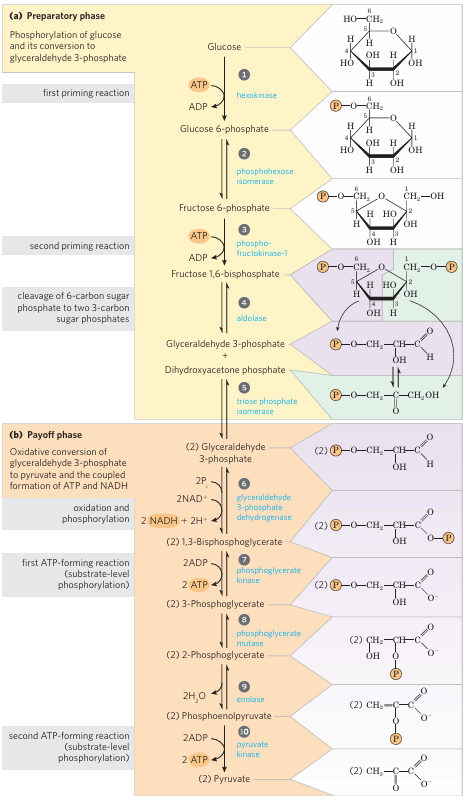
\includegraphics[width = 0.5 \textwidth]{glycolysis_gen}
	\caption{Glycolysis}
\end{figure}
\begin{itemize}
	\item \textbf{Glucose} + 2ADP + 2NAD+ + 2Pi => \textbf{2 Pyruvate + 2ATP + 2NADH} + 2 H+ + 2 H2O
\end{itemize}

\paragraph{Carbon labeling}
Note when labeling GA3P the number do not correspond to the same numbers from the fructose compound. \textit{One always follows the normal rules}
\begin{figure}[H]
	\centering
	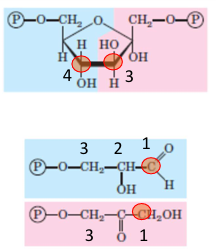
\includegraphics[height = 5cm]{labeling}
	\caption{Carbon labeling}
\end{figure}

Glycolysis can be dived in two stages the preparation phase and the payoff phase. 

\subsubsection{Stage 1, Preparation Phase}
In the preparation phase glucose gets \textbf{trapped} inside the cell, "\textbf{activated}", and \textbf{broken down} into smaller components.  
\paragraph{Step1: Posphorylation of Glucose}
\textbf{D-Glucose} moves into the cell with the help of a \textbf{membrane transporter}. Once in the cytoplasma it undergoes phosporylation by \textbf{hexokinase} to produce \textbf{Glucose 6-phosphate}. This has two consequences: 
\begin{itemize}
	\item \textbf{No backsies}: Glucose 6-phosphate is structurally different and thus can not be transported out by the same membrane transporter. 
	\item \textbf{More reactive}: The substitution of the hydroxy group with the phosphate group (2 addition charges, etc.) makes the molecule more reactive. But this has to be payed by the \textbf{investment} of 1 ATP molecule.
\end{itemize}

\begin{figure}[H]
	\centering
	\subfigure[Step 1]{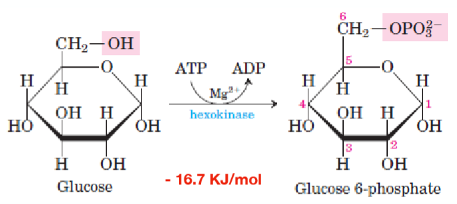
\includegraphics[width = 0.6 \textwidth]{S1}}
	\subfigure[Hexokinase]{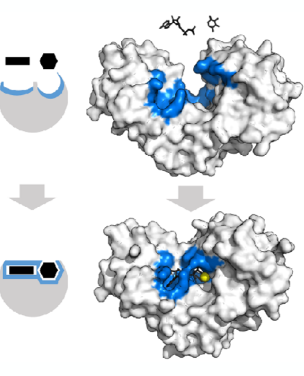
\includegraphics[width = 0.25 \textwidth]{HK}\label{HK}}
	\caption{Posphorylation of Glucose}
\end{figure}

\begin{RemarkWithTitel}{Hexokinase (HK)}
	\gls{hexokinase} is an enzyme that phosphorylates hexoses (like glucose) using ATP. Like most kinases it requires the presence of the cofactor Mg2+ in the active site. \\
	The movement of Glucose into HK active site causes a conformational change wherby two HK lobes roted by 12 defrees (10 $\AA$) creating an \textbf{induced fit}. This makes the \textbf{carbon 6 oriented towards ATP} and squeezes out water molecules. (see fig. \ref{HK}) 
\end{RemarkWithTitel}

\paragraph{Step2: Isomerization}
In the second step the enzyme \textbf{phospho-glucose isomerase} transforms alsose (Glucose) into ketose (Fructose). This is done in order to create more symmetry preparing step 3. 

\begin{figure}[H]
	\centering
	\subfigure[6 to 5 ring]{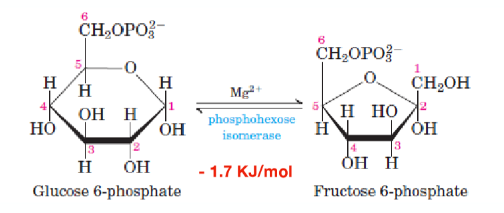
\includegraphics[width = 0.6 \textwidth]{S2_1}}
	\subfigure[aldose to ketose]{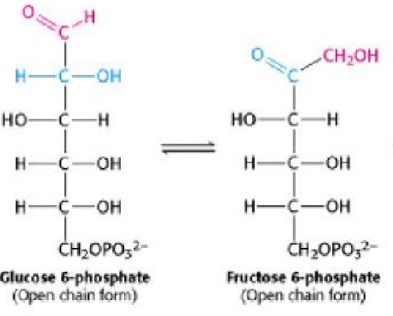
\includegraphics[width = 0.3 \textwidth]{S2_2}}
	\caption{Isomerization}
\end{figure}

\paragraph{Step3: Second phosphorylation}
The enuyme \textbf{phospho-fructo kinase-1 (PFK-1)} turns Fructose 6-phophate into Fructiose 1,6-biphosphate, completing the symmetry and making the compound even more reactive. This is again paid with the \textbf{investment of 1 ATP}. (see fig. \ref{S3})\\
\\
Note, that \textbf{this step commits the sugar to glycolysis}. This is why \textbf{PFK-1 is a highly regulated enzyme} where its activity is modified according to cellular concentration of ATP, ADP, and AMP. (\textbf{ATP inhibits - AMP stimulates}). 

\paragraph{Step4: Breakdown of Fructose 1,6-biphosphate}
\textbf{Aldolase} catalyses the breakdown of Fructose 1,6-biphosphate into 2 different three-carbon molecules (\textbf{GA3P and DHAP}). 
\begin{figure}[h!]
	\centering
	\subfigure[creation of perfect symmetry]{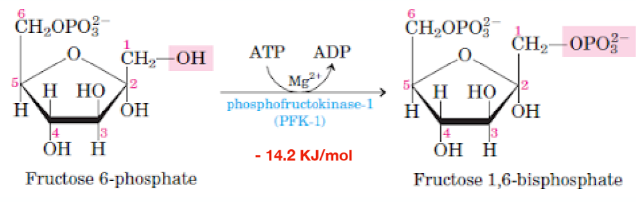
\includegraphics[width = 0.45 \textwidth]{S3}\label{S3}}
	\subfigure[breakdown]{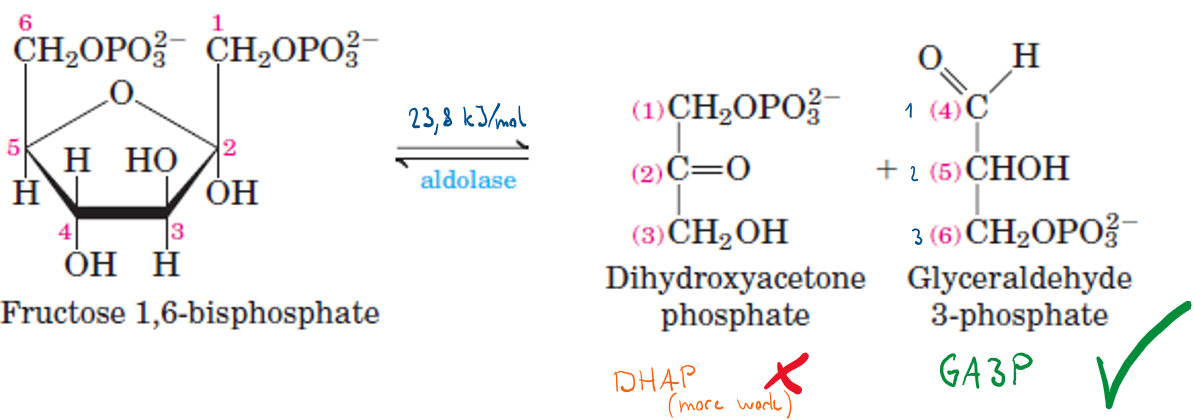
\includegraphics[width = 0.45 \textwidth]{S4}}
	\caption{Step3 and Step4}
\end{figure}
GA3P feeds directely in the glycolytic pathway without any further change while DHAP needs to be first transformed.  This is archived by Step5. 
\paragraph{Step5: Isomerisation of DHAP to GA3P}
\textbf{Triose phosphate isomerase (TPI or TIM)} catalyses the rapid and reversible conversion of DAHP to GA3P, ketone to aldehyde. This happens via an intramolecular redox reactimon where \textbf{an hydrogen is transferred from C1 to C2}.
\begin{figure}[H]
	\centering
	\subfigure[Step5]{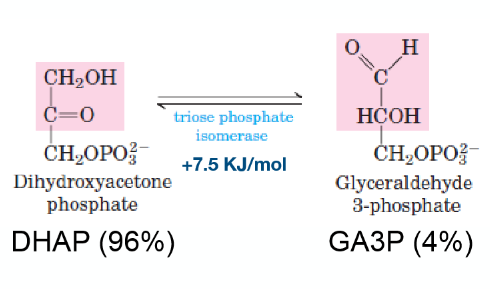
\includegraphics[width = 0.3 \textwidth]{S5_1}}
	\subfigure[Mechanism of TIP]{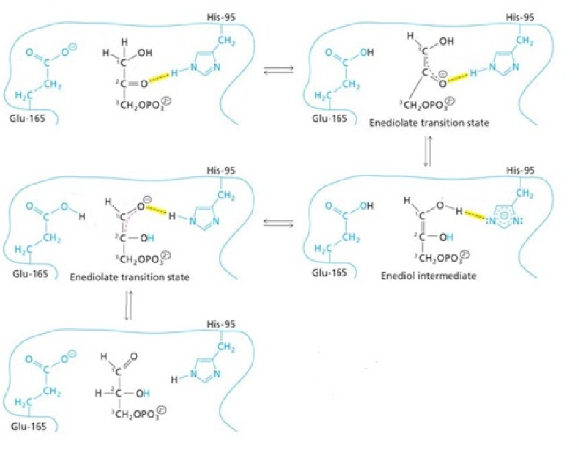
\includegraphics[width = 0.6 \textwidth]{S5_2}}
	\caption{Isomerisation of DHAP to GA3P}
\end{figure}
Even though TIP increases the rate by 10 billion fold the equilibrium still lies on the unwanted side of DHAP (the \textbf{reaction is unfavorable}). But since the reaction is coupled to endorgenic reactions (GA3P is always directely used), \textbf{the reaction shifts to the side of the product GA3P}.  

\subsubsection{Stage2, Payoff Phase}
In the payoff phase the components from the stage 1 get \textbf{oxidized} in order to produce ATP, NADH, and pyruvat. 

\paragraph{Step6: Conversion of GA3P to 1,3-BPG}
GA3P is converted into 1,3-biphosphoglycerate (1,3-BPG) by the enzyme glyceraldehyde 3-phophate \textbf{dehydrogenase (GAPDH)}. Note this reaction produces NADH, which can later be oxidized.  
\begin{figure}[H]
	\centering
	\subfigure[Step6]{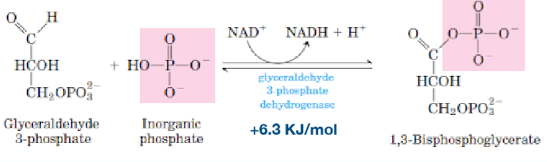
\includegraphics[width = 0.3 \textwidth]{S6_1}}
	\subfigure[Mechanism of GAPDH]{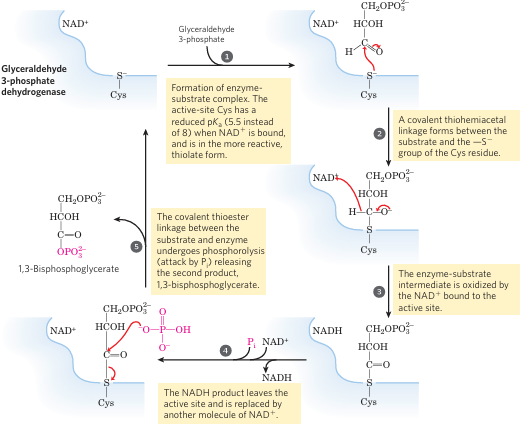
\includegraphics[width = 0.6 \textwidth]{S6_2}}
	\caption{Conversion of GA3P to 1,3-BPG}
\end{figure}
\paragraph{Step7: Phosphotransfer from 1,3-BPG to ADP}
Step7 is the \textbf{break-even point}. 1, 3-BPG is used as a phophate doner to ADP. This reaction is catalyzed by \textbf{glycerophophate kinase} and produces 3-Phophoglycerate and ATP. (see fig. \ref{S7})

\paragraph{Step8: Conversion to 2-Phophopglycerate}
\textbf{Phophoglycrate mutase} catalyses the transfer of the phosphate group from C3 of 3-phosphoglycerate to C2 to form 2-phosphoglycerate. 

\begin{figure}[h!]
	\centering
	\subfigure[Break-Even point]{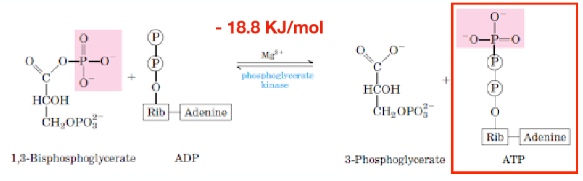
\includegraphics[width = 0.45 \textwidth]{S7}\label{S7}}
	\subfigure[Repositioning of Phosphate group]{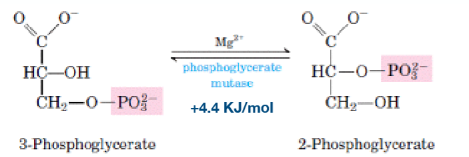
\includegraphics[width = 0.45 \textwidth]{S8}}
	\caption{Step7 and Step8}
\end{figure}

\paragraph{Step9: Conversion to Phophoenolpyruvate (PEP)}
\textbf{Enolase} converts 2-phosphoglycerate into  posphoenolpyruvate (PEP). This \textbf{dehydration reaction increases the phosphoryltransfer potential} of the molecule.

\paragraph{Step10: Conversion to Pyruvate}
The phosphoryltransfer potential of \textbf{PEP} is exploited to create ATP and pyruvate. The enzyme \textbf{pyruvate kinase} catalyses the phosphoric transfer. At this point we have gained a \textbf{total of 2 ATP and 2 NADH}. 
\begin{figure}[h!]
	\centering
	\subfigure[Dehydration by enolase]{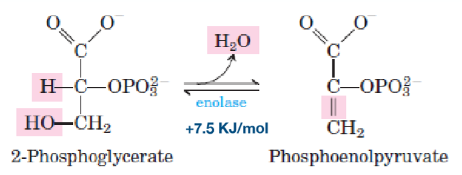
\includegraphics[width = 0.45 \textwidth]{S9}\label{S9}}
	\subfigure[Gain of 2 ATP and 2 Pyruvate]{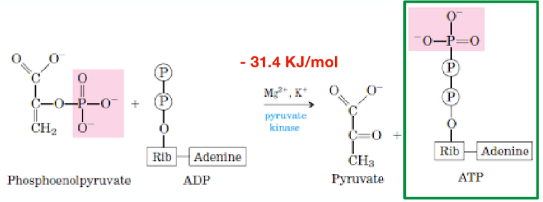
\includegraphics[width = 0.45 \textwidth]{S10}}
	\caption{Step9 and Step10}
\end{figure}

\subsubsection{The fates of Pyruvate}
\gls{pyruvate} is a three-carbon molecule that is the end product of glycolysis.

\begin{figure}[H]
	\centering
	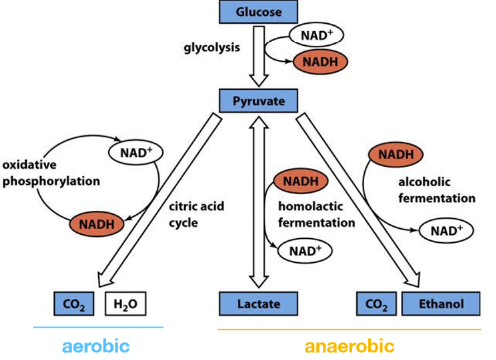
\includegraphics[width = 0.7 \textwidth]{fate_of_pyruvate}
	\caption{The fates of Pyruvate}
\end{figure}

\begin{DefWithTitle}{Facultative Anaerobic Organism}
	A \gls{fanaerorg} is able to produce ATP by anerobic respiration if oxygen is present, but is also capable of switching to fermentation if oxygen is absent. For example E.coli or some muscle cells (temporarily in humans). 
\end{DefWithTitle}

\begin{RemarkWithTitel}{Soy Sauce}
	Soy sauce is produced by \textbf{fermenting a salted mixture of soy beans}. Soybeans contain starch whcih will be broken down to glucose and then degradated via glycolysis to pyruvate. And the fermented in the absence of oxygen. However \textbf{if oxygen were present} pyruvate would be oxydized to acetyl-CoA entering the citric acid cycle. But some a\textbf{cetyl-CoA would get hydrolyzed to acetic acid (vinegar)} which would result in a undesired strong vinegar taste.
\end{RemarkWithTitel}

\paragraph{Ethanol Fermentation}
\textbf{Yeast} and sveral bacteria utilise ethanol (alcoholic) fermentation to \textbf{regenerate NAD+} and to transform pyruvate into \textbf{ethanol and carbon dioxide}.\\
\\
In a first step \textbf{pyruvate decarboxylase} catalyses a decarboxylation reaction. The enzymes needs the\textbf{ coenzyme TPP}, a vitamin B1 derivative, and cofactor Mg2+ 
\begin{itemize}
	\item Note, that the \textbf{C3 \& C4 carbons of glucose will be cut away} in form of CO2. 
\end{itemize}
In the second step \textbf{alcohol dehydrogenase} will regenerate NAD+ in reducing acetaldehyde to ethanol. Note alcohol dehydrogenase conatins a \textbf{zinc ion} in the active site to help polarize the carbonyl double bond that promotes hybride transfer from NADH. 

\begin{figure}[H]
	\centering
	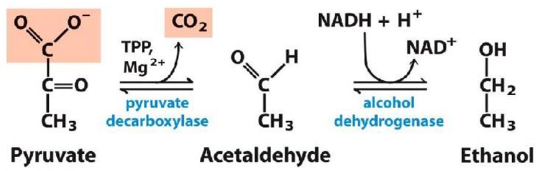
\includegraphics[width = 0.6 \textwidth]{ethanol}
	\caption{Ethanol Fermentation}
\end{figure}

\begin{itemize}
	\item Glucose + 2ADP + 2Pi => 2 Ethanol + \textbf{2ATP} + 2 CO2 + 2 H2O
\end{itemize}

\paragraph{Lactic Fermentation}
\textbf{Many prokaryotic and eukaryotic} organisms can use lactic fermentation. Like ethanol fermentation it is nessesary to \textbf{regenerate NAD+}. Lactic fermentation is catalysed by \textbf{lactate dehydrogenase (LHD)}. 

\begin{figure}[H]
	\centering
	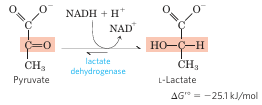
\includegraphics[width = 0.6 \textwidth]{lactic}
	\caption{Lactic Fermentation}
\end{figure}

\begin{RemarkWithTitel}{Cancer, PET scan}
	Cancer cells often rely on aerobic glycolysis, known as the\textbf{ Warburg effect}, where they preferentially use glycolysis followed by lactic acid fermentation, even in the presence of oxygen. This allows them to rapidly generate ATP and biosynthetic precursors for growth.\\
	Positron Emission Tomography (PET scans) exploit this metabolic shift by using \textbf{fluorodeoxyglucose (FDG)}, a radiolabeled glucose analog. Since cancer cells have a higher glucose uptake due to increased glycolysis, they accumulate FDG, which emits positrons detectable by \textbf{PET imaging}.
	
\end{RemarkWithTitel}


\subsection{TCA cycle}

\paragraph{Pyruvate => Acetyl-CoA}

\subsubsection{TCA cylce steps}

\paragraph{Step1}

\paragraph{Step2}

\paragraph{Step3}

\paragraph{Step4}

\paragraph{Step5}

\paragraph{Step6}

\paragraph{Step7}

\paragraph{Step8}

\begin{RemarkWithTitel}{What happens to 3-14C-pyruvate}
	use nice picture with correct labelling of ocalacetate. 
\end{RemarkWithTitel}


\subsection{Fatty Acid Oxidation}

\paragraph{What about glycerol?}

\paragraph{Transport within Mitochondria}

make glossary entry for carnitine 

\begin{RemarkWithTitel}{Primary Carnitine deficiency}
	Inhalt...
\end{RemarkWithTitel}

\subsubsection{Beta oxidation}
During beta-oxidation, each cycle shortens the fatty acid chain by 2 carbon atoms, producing 1 molecule of acetyl-CoA per cycle.

How to calculate how many ATP from a FAs of given lenght. 

What if usaturated FA 

What if odd number of carbons:


ChatGPT saysy (for the 3 rest)


The short answer is that it produces less ATP. When a fatty acid has an odd number of carbons, the final 3‐carbon fragment is converted into propionyl‐CoA, which is then converted into succinyl‐CoA. This conversion requires an ATP investment and bypasses the early steps of the TCA cycle that normally generate additional reducing equivalents (NADH). As a result, while a full acetyl‐CoA oxidation (entering the TCA cycle from the start) yields about 10 ATP, succinyl‐CoA—entering mid‐cycle—yields roughly 5 ATP (and even a bit less when you factor in the ATP cost of converting propionyl‐CoA to succinyl‐CoA).

So overall, the energy yield from the odd-chain fatty acid’s final three carbons is lower compared to that of a full acetyl‐CoA molecule.

\paragraph{Step1}

\paragraph{Step2}

\paragraph{Step3}

\paragraph{Step4}

\subsection{unsaturated FAs}

\subsection{Amino Acid Oxidation}

\subsubsection{Urea production}

\subsubsection{Entry in CAC}

\paragraph{Phenylalanine catabolism}















\subsection{ECT}


\end{document}